\chapter{Bài toán sắp xếp}
Khi so sánh các thuật toán sắp xếp, ta quan tâm tới một số điều:
\begin{itemize}
    \item \textbf{Thời gian chạy}: với lượng dữ liệu lớn máy sẽ mất rất nhiều thời gian để chạy, không thể sử dụng trong thực tế.
    \item \textbf{Bộ nhớ}: đối với các hệ thống bộ nhớ thấp (hệ thống nhúng), một vài thuật toán sẽ không thể chạy được.
    \item \textbf{Tính ổn định}: Đối với thuật toán sắp xếp ổn định, các phần tử có giá trị bằng nhau sẽ giữ nguyên thứ tự như trước khi sắp xếp. Tính ổn định có vai trò quan trọng khi ta sắp xếp nhiều lần để tuân theo nhiều tiêu chí.
\end{itemize}
Trong khuôn khổ chương này, chỉ có thuật toán Bubble Sort, Insertion Sort và Merge Sort là ổn định. Về minh hoạ, trừ Heap Sort ra bạn đều có thể đến \href{https://visualgo.net/en/sorting}{VisualAlgo}.

\section{Thuật toán Bubble Sort}
Cho dãy S với n phần tử cần được sắp xếp tăng dần. Xét các phần tử $a_i$ và $a_{i+1}$. Nếu $a_i>a_{i+1}$, ta đổi chỗ hai phần tử. Nói cách khác, phần tử nhỏ nhất sẽ \textbf{nổi} lên trên, vì vậy đây còn được gọi là thuật toán sắp xếp nổi bọt. Lặp lại đến khi không còn 2 phần tử nào thoả mãn.

\begin{minted}{cpp}
for (int i = 0; i < n; i++)
    for (int j = 0; j < n - 1; j++)
        if (a[j] > a[j + 1])
            swap(a[j], a[j + 1]);
\end{minted}

Dễ thấy rằng sau mỗi vòng lặp của i, các phần tử cần được sắp xếp sẽ được dịch chuyển 1 vị trí. Vậy trong trường hợp xấu nhất (phần tử lớn nhất nằm ở đầu dãy hoặc phần tử nhỏ nhất ở cuối dãy), cả n vòng lặp i đều sẽ được dùng để đưa phần tử này về đúng vị trí. Các trường hợp còn lại sẽ không dùng tới toàn bộ n vòng lặp, nhưng để đảm bảo, ta lặp đến n cho i. Vậy độ phức tạp thời gian là $O(n^2)$, độ phức tạp bộ nhớ là $O(1)$.
\section{Thuật toán Insertion Sort}
Ý tưởng của thuật toán này là sẽ đưa từng phần tử một về đúng vị trí của nó trong dãy. Giả sử dãy đã có i phần tử được sắp xếp, ta tìm chỗ cho phần tử thứ i + 1 và \textbf{chèn} nó vào đó. Vì vậy đây còn được gọi là thuật toán sắp xếp chèn.

Ta thấy rằng khi dãy đã gần được sắp xếp xong, Insertion Sort sẽ chạy rất nhanh, ví dụ như sắp xếp điểm cao trong game.

\begin{minted}{cpp}
for (int i = 1; i < N; i++) {
    // Tìm vị trí phù hợp cho S[i] bằng tìm kiếm nhị phân
    int l = 0, r = i - 1;
    while (l <= r) {
        int m = (l + r) / 2;
        if (S[m] < S[i])
            l = m + 1;
        else
            r = m - 1;
    }
    // Đưa S[i] về vị trí l (dời dãy)
    int tmp = S[i];
    for (int k = i; k > l; k--)
        S[k] = S[k - 1];
    S[l] = tmp;
}
\end{minted}

Đánh giá về độ phức tạp, dễ thấy rằng ta cần 1 vòng lặp để duyệt qua mọi phần tử, và 1 vòng lặp nữa để đưa nó về đúng vị trí (ta chỉ quan tâm đến độ phức tạp lớn nhất trong vòng lặp, trong trường hợp này là $O(n)$). Trong trường hợp xấu nhất như Bubble Sort, vòng lặp này sẽ có độ phức tạp $O(n)$. Vậy độ phức tạp thời gian là $O(n)$, độ phức tạp bộ nhớ là $O(1)$.

\section{Thuật toán Shell Sort - Insertion Sort cải tiến}
Nhược điểm của Insertion Sort là sẽ mất rất nhiều thao tác để ta có thể chèn phần tử vào vị trí gần đầu dãy. Shell Sort tối ưu hoá theo tư tưởng chia dãy số thành nhiều dãy con, với dãy con $S_1=\{S_0,S_{h},S_{2h}\dots\},S_2=\{S_1,S_{1+h},S_{1+2h}\dots\}\dots$ với h là bước, ta có thể chọn h sao cho phù hợp. Ví dụ với dãy (4, 6, 7, 2, 3, 5, 1, 9, 8), h = 3:

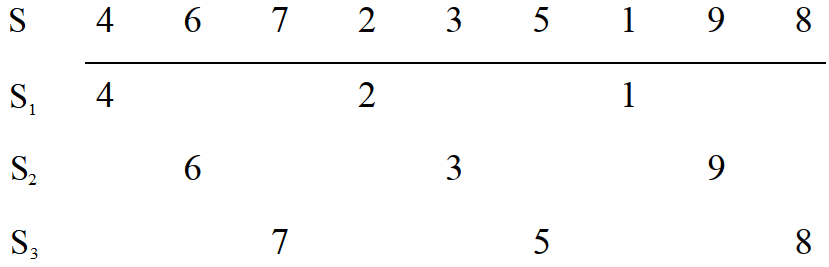
\includegraphics[scale=0.45]{sapxep/shellsort.png}

Dễ thấy rằng ở thao tác dời dãy, phần tử $S_6=1$ thay vì phải thao tác trên 6 phần tử trước nó thì giờ đây chỉ cần thao tác qua 2 phần tử, nhanh chóng được đưa về vị trí \textbf{gần đúng} của nó. Để tăng độ chính xác (tìm vị trí chính xác), ta chia đôi h đến khi h = 1 (có nghĩa là gộp 2 dãy con lại), ta được dãy sắp xếp.

\section{Thuật toán Heap Sort}
Trong khuôn khổ này, heap đơn giản là một cây nhị phân với nút cha mang giá trị lớn hơn 2 nút con.

Nếu vậy, nút gốc sẽ mang giá trị lớn nhất trong dãy. Vậy ta sẽ lấy giá trị nút gốc cho vào cuối dãy, sau đó xoá nút gốc đi, đưa nút lá cuối cùng lên gốc, lúc này heap không còn đúng nữa, ta sẽ đảo các nút sao cho đúng thứ tự trở lại, việc này gọi là \textbf{vun đống heap}, vì vậy đây còn được gọi là thuật toán sắp xếp vun đống. Lặp lại đến khi heap rỗng.

Khi sắp xếp tăng dần, ta thu được một cây, trong đó nút gốc là phần tử lớn nhất của dãy, hay còn gọi là \textbf{max heap}, ngược lại với \textbf{min heap}.

Ví dụ với dãy S = [4, 7, 3, 5, 2, 6, 1]. Hình bên trái là cây nhị phân sau khi xây, bên phải là sau khi được vun đống.

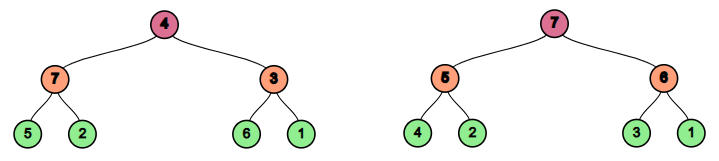
\includegraphics[scale=0.55]{sapxep/heapify}

Độ phức tạp thời gian là $O(n\log_2n)$ vì ta phải vun đống $n$ lần, vì vun đống duyệt theo chiều cao của cây, tối đa là $\log_2n$. Độ phức tạp bộ nhớ là $O(1)$.

\section{Thuật toán Quick Sort}
Ta chia dãy thành 2 phần, một phần "lớn" và một phần "nhỏ" bằng cách chọn một phần tử chốt (hay gọi là \textbf{pivot}), đưa nó về đúng vị trí bằng Insertion Sort, tiếp tục gọi đệ quy cho từng phần đến khi mỗi phần chỉ còn 2 phần tử (điều kiện dừng đệ quy) và sắp xếp 2 phần tử.

Thuật toán này nổi tiếng vì nó chạy nhanh nhất trong tất cả các thuật toán sắp xếp dựa theo so sánh (tác giả của nó đã tự tin đặt cho nó cái tên Quick Sort - sắp xếp nhanh), được sử dụng nhiều trong các thư viện của Java, C++ (hàm \texttt{sort} của C++ dùng Intro Sort là kết hợp giữa Quick Sort và Insertion Sort).

Tuy nhiên, ta thấy rằng độ phức tạp thời gian có phần ngẫu nhiên, phụ thuộc vào cách chọn \textbf{pivot}, nếu tất cả pivot được chọn đều trong trường hợp xấu nhất như trên, độ phức tạp sẽ tương đương với Insertion Sort $O(n^2)$, nhưng trong trường hợp ngẫu nhiên, trung bình là $O(n\log_2n)$ (ta chia đôi dãy sau mỗi lần gọi đệ quy, vậy có tối đa $\log_2n$ lần chia).

\begin{minted}{cpp}
void quickSort(int* S, int l, int r) {
    // điều kiện dừng đệ quy
    if (l >= r) return;
    
    int i = l, j = r;
    int pivot = S[l + rand() % (r - l + 1)];

    // đưa pivot về đúng vị trí
    while (i <= j) {
        while (S[i] < pivot) i++;
        while (S[j] > pivot) j--;
        if (i <= j) {
            std::swap(S[i], S[j]);
            i++; j--;
        }
    }

    // gọi đệ quy sắp xếp phần bên trái
    quickSort(S, l, j);
    // gọi đệ quy sắp xếp phần bên phải
    quickSort(S, i, r);
}
\end{minted}

Phân tích về chọn ngẫu nhiên pivot, một số ví dụ sau đây sẽ làm Quick Sort bị suy biến:
\begin{itemize}
    \item pivot = $S_0$ (phần tử đầu tiên) hoặc pivot = $S_n$ (phần tử cuối cùng) thì dễ thấy rằng nó sẽ gọi đệ quy cho phần bên phải/trái liên tục $n$ lần, gây ra độ phức tạp $O(n^2)$.
    \item pivot = $S_m$ (phần tử giữa), với m lớn thì nó cũng bị suy biến.
\end{itemize}
Vậy cách tốt nhất là chọn ngẫu nhiên để trung bình hoá các lần chọn tốt và lần chọn không tốt nhằm chạy với độ phức tạp trung bình.

\section{Thuật toán Merge Sort}
Thuật toán sắp xếp đệ quy này chia đôi dãy số, so sánh hai phần tử của nó và trộn lại nên được gọi là thuật toán \textbf{sắp xếp trộn}.

Đầu tiên ta tạo một mảng S' khác để lưu mảng đã sắp xếp.

Ta chia đôi dãy số (gọi đệ quy đến khi dãy con chỉ còn 1 phần tử), so sánh hai phần tử đầu tiên của hai phần. Phần tử nhỏ hơn ta cho vào S' và xoá khỏi phần tương ứng. Tiếp tục so sánh bằng vòng lặp đến khi đã cho hết hai dãy vào S', Sao chép dữ liệu trở lại dãy S và lặp lại đến khi sắp xếp xong.

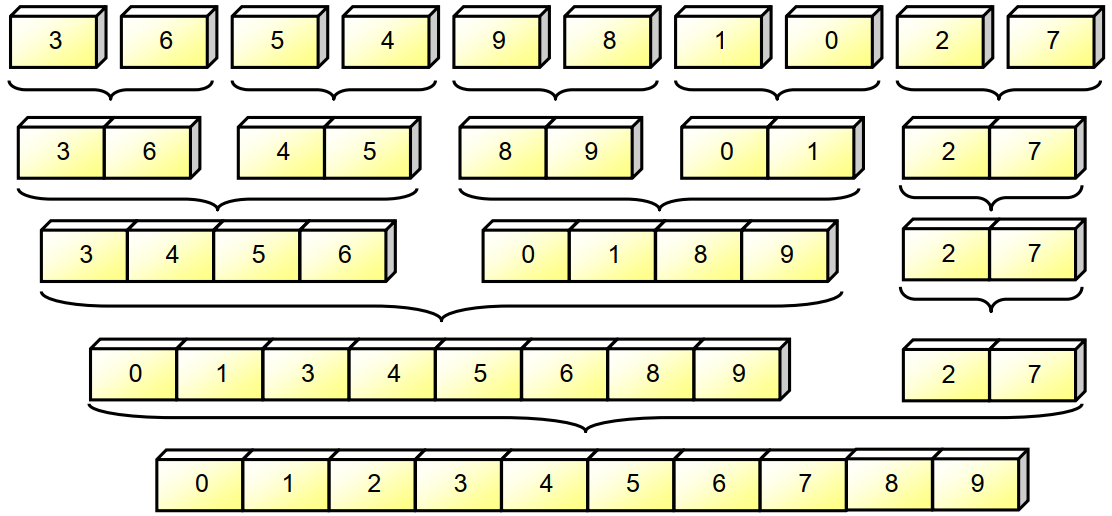
\includegraphics[scale=0.35]{sapxep/mergesort.png}

Độ phức tạp thời gian tương tự như Quick Sort $O(n\log_2n)$ nhưng độ phức tạp bộ nhớ là $O(n)$ do mảng S'.

\begin{minted}{cpp}
// giả sử N là số phần tử
int S_[N]; // S'

void mergeSort(int* S, int l, int r) {
    // dãy chỉ gồm 1 phần tử, điều kiện dừng đệ quy
    if (l >= r) return;
    // chia đôi dãy
    int m = l + (r - l) / 2;
    // gọi đệ quy chia đôi
    mergeSort(S, l, m);
    mergeSort(S, m + 1, r);
    // bắt đầu so sánh
    int i = l, j = m + 1;
    int cur = 0; // vị trí phần tử trong S'
    while (i <= m || j <= r) {
        // bên trái không còn phần tử nào
        if (i > m)
            S_[cur++] = S[j++];
        // bên phải không còn phần tử nào
        else if (j > r)
            S_[cur++] = S[i++];
        // phần tử bên trái nhỏ hơn
        else if (S[i] < S[j])
            S_[cur++] = S[i++];
        else
            S_[cur++] = S[j++];
    }
    // copy mảng S_ trở lại S
    for (int k = 0; k < cur; k++)
        S[l + k] = S_[k];
}
\end{minted}

\section{Thuật toán Radix Sort}
Thuật toán này đặc biệt hơn các thuật toán khác ở chỗ, nó không sắp xếp theo so sánh số, nhưng sắp xếp theo so sánh chữ số của các số đó, nên được gọi là thuật toán so sánh \textbf{theo cơ số}.

Ta chia các phần tử theo các nhóm (dựa theo bit đầu tiên, chữ số đầu tiên\dots). Sắp xếp lại chúng theo nhóm. Tiếp tục chia nhỏ hơn đến khi đến bit/chữ số cuối cùng.

Ví dụ với S = [1, 3, 7, 6, 5, 2, 3, 4, 4, 5, 6, 7]:

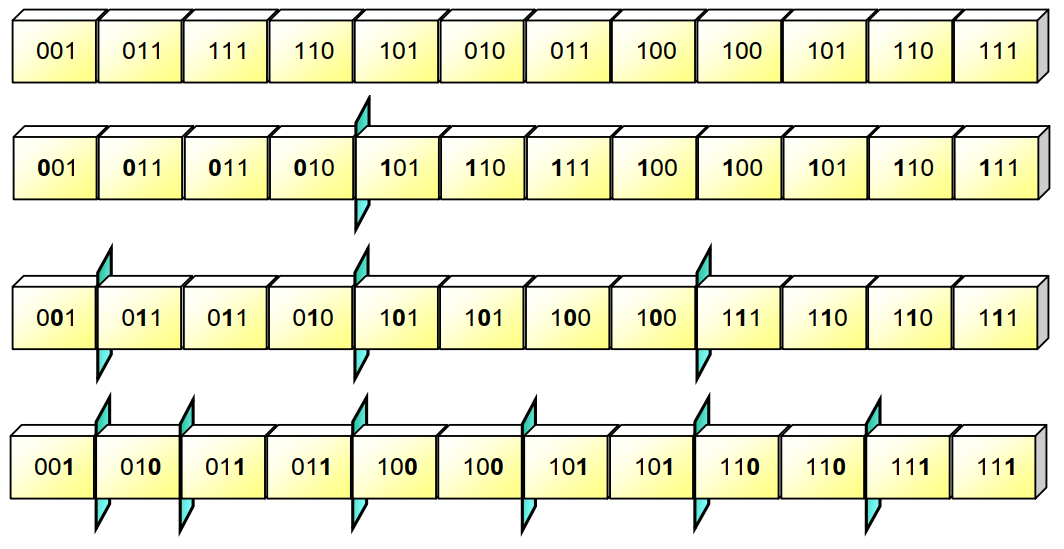
\includegraphics[scale=0.35]{sapxep/radixSort.png}

Thuật toán này chạy nhanh hơn các thuật toán khác, với độ phức tạp thời gian là $O(n.\log_k(\max(S)))$ với $\max(S)$ là phần tử lớn nhất của S, k là cơ số, ví dụ nếu chia theo từng bit, số $S_i$ có $\log_2(S_i)$ bit hay k = 2, nếu chia theo từng chữ số, thì có $\log(S_i)$ chữ số hay k = 10.

\section{Sắp xếp bằng cách đếm phân phối}
Nếu dãy S là một dãy có nhiều phần tử trùng lặp, thuật toán này sẽ hoạt động rất nhanh.

Tư tưởng của nó là ta đếm số lần xuất hiện của từng giá trị, sau đó duyệt qua các giá trị từ nhỏ tới lớn (không cần sắp xếp vì ta có thể dùng mảng để đánh dấu số lần, duyệt qua các chỉ số từ nhỏ đến lớn, nếu số lớn ta có thể nén số), thêm lần lượt các giá trị trở lại dãy.

Dễ thấy rằng ta cần duyệt qua dãy mất n thao tác, sau đó duyệt qua số lượng giá trị riêng biệt mất M thao tác, hay độ phức tạp $O(M + n)$, độ phức tạp bộ nhớ $O(M)$.